{applications,approximation,discrete,namd,performance,programming}.texDense linear algebra, that is linear algebra on matrices that are
stored as two-dimensional arrays (as opposed to sparse linear algebra;
see section~\ref{sec:sparse}, as well as the
tutorial on PETSc~\ref{tut:petsc}) has been standardized for a
considerable time. The basic operations are defined by the three
levels of \indexac{BLAS}:
\begin{itemize}
\item Level~1 defines vector operations that are characterized by a
  single loop~\cite{Lawson:blas}.
\item Level~2 defines matrix vector operations, both explicit such as
  the matrix-vector product, and implicit such as the solution of
  triangular systems~\cite{BLAS2}.
\item Level~3 defines matrix-matrix operations, most notably the
  matrix-matrix product~\cite{BLAS3}.
\end{itemize}
The name `BLAS' suggests a certain amount of generality, but the
original authors were clear~\cite{Lawson:blas} that these subprograms
only covered dense linear algebra. Attempts to standardize sparse
operations have never met with equal success.

Based on these building blocks libraries have been built that tackle
the more sophisticated problems such as solving linear systems, or
computing eigenvalues or singular values.
\indexterm{Linpack}\footnote{The linear system solver from this
  package later became the \indextermbus{Linpack}{benchmark}; see
  section~\ref{sec:top500}.} and \indexterm{Eispack} were the first to formalize
these operations involved, using Blas Level~1 and Blas Level~2
respectively.  A~later development, \indexterm{Lapack} uses the
blocked operations of Blas Level~3. As you saw in
section~\ref{sec:reuse}, this is needed to get high performance on
cache-based CPUs. (Note: the reference implementation of the
BLAS~\cite{reference-blas} will not give good performance with any
compiler; most platforms have vendor-optimized implementations, such
as the \indexterm{MKL} library from Intel.)

With the advent of parallel computers, several projects arose that
extended the Lapack functionality to distributed computing, most
notably \indexterm{Scalapack}~\cite{scalapack} and
\indexterm{PLapack}~\cite{PLAPACK,PLAPACK:UG}. These packages are
considerably harder to use than Lapack\footnote{PLapack is probably
  the easier to use of the two.} because of the need for the
two-dimensional block cyclic distribution; sections
\ref{sec:densescaling} and~\ref{sec:LUscaling}. We will not go into
the details here.

\Level 1 {BLAS matrix storage}

There are a few points to bear in mind about the way matrices are
stored in the BLAS and LAPACK\footnote{We are not going into band
  storage here.}:

\Level 2 {Array indexing}

Since these libraries originated in a Fortran environment, they
  use 1-based indexing. Users of languages such as C/C++ are only
  affected by this when routines use index arrays, such as the
  location of pivots in LU factorizations.

\Level 2 {Fortran column-major ordering}

Since computer memory is one-dimensional, some conversion is needed
from two-dimensional matrix coordinates to memory locations. The
\indexterm{Fortran} language uses \indexterm{column-major} storage, that is,
elements in a column are stored consecutively; see
figure~\ref{fig:densearray}.
\begin{figure}
  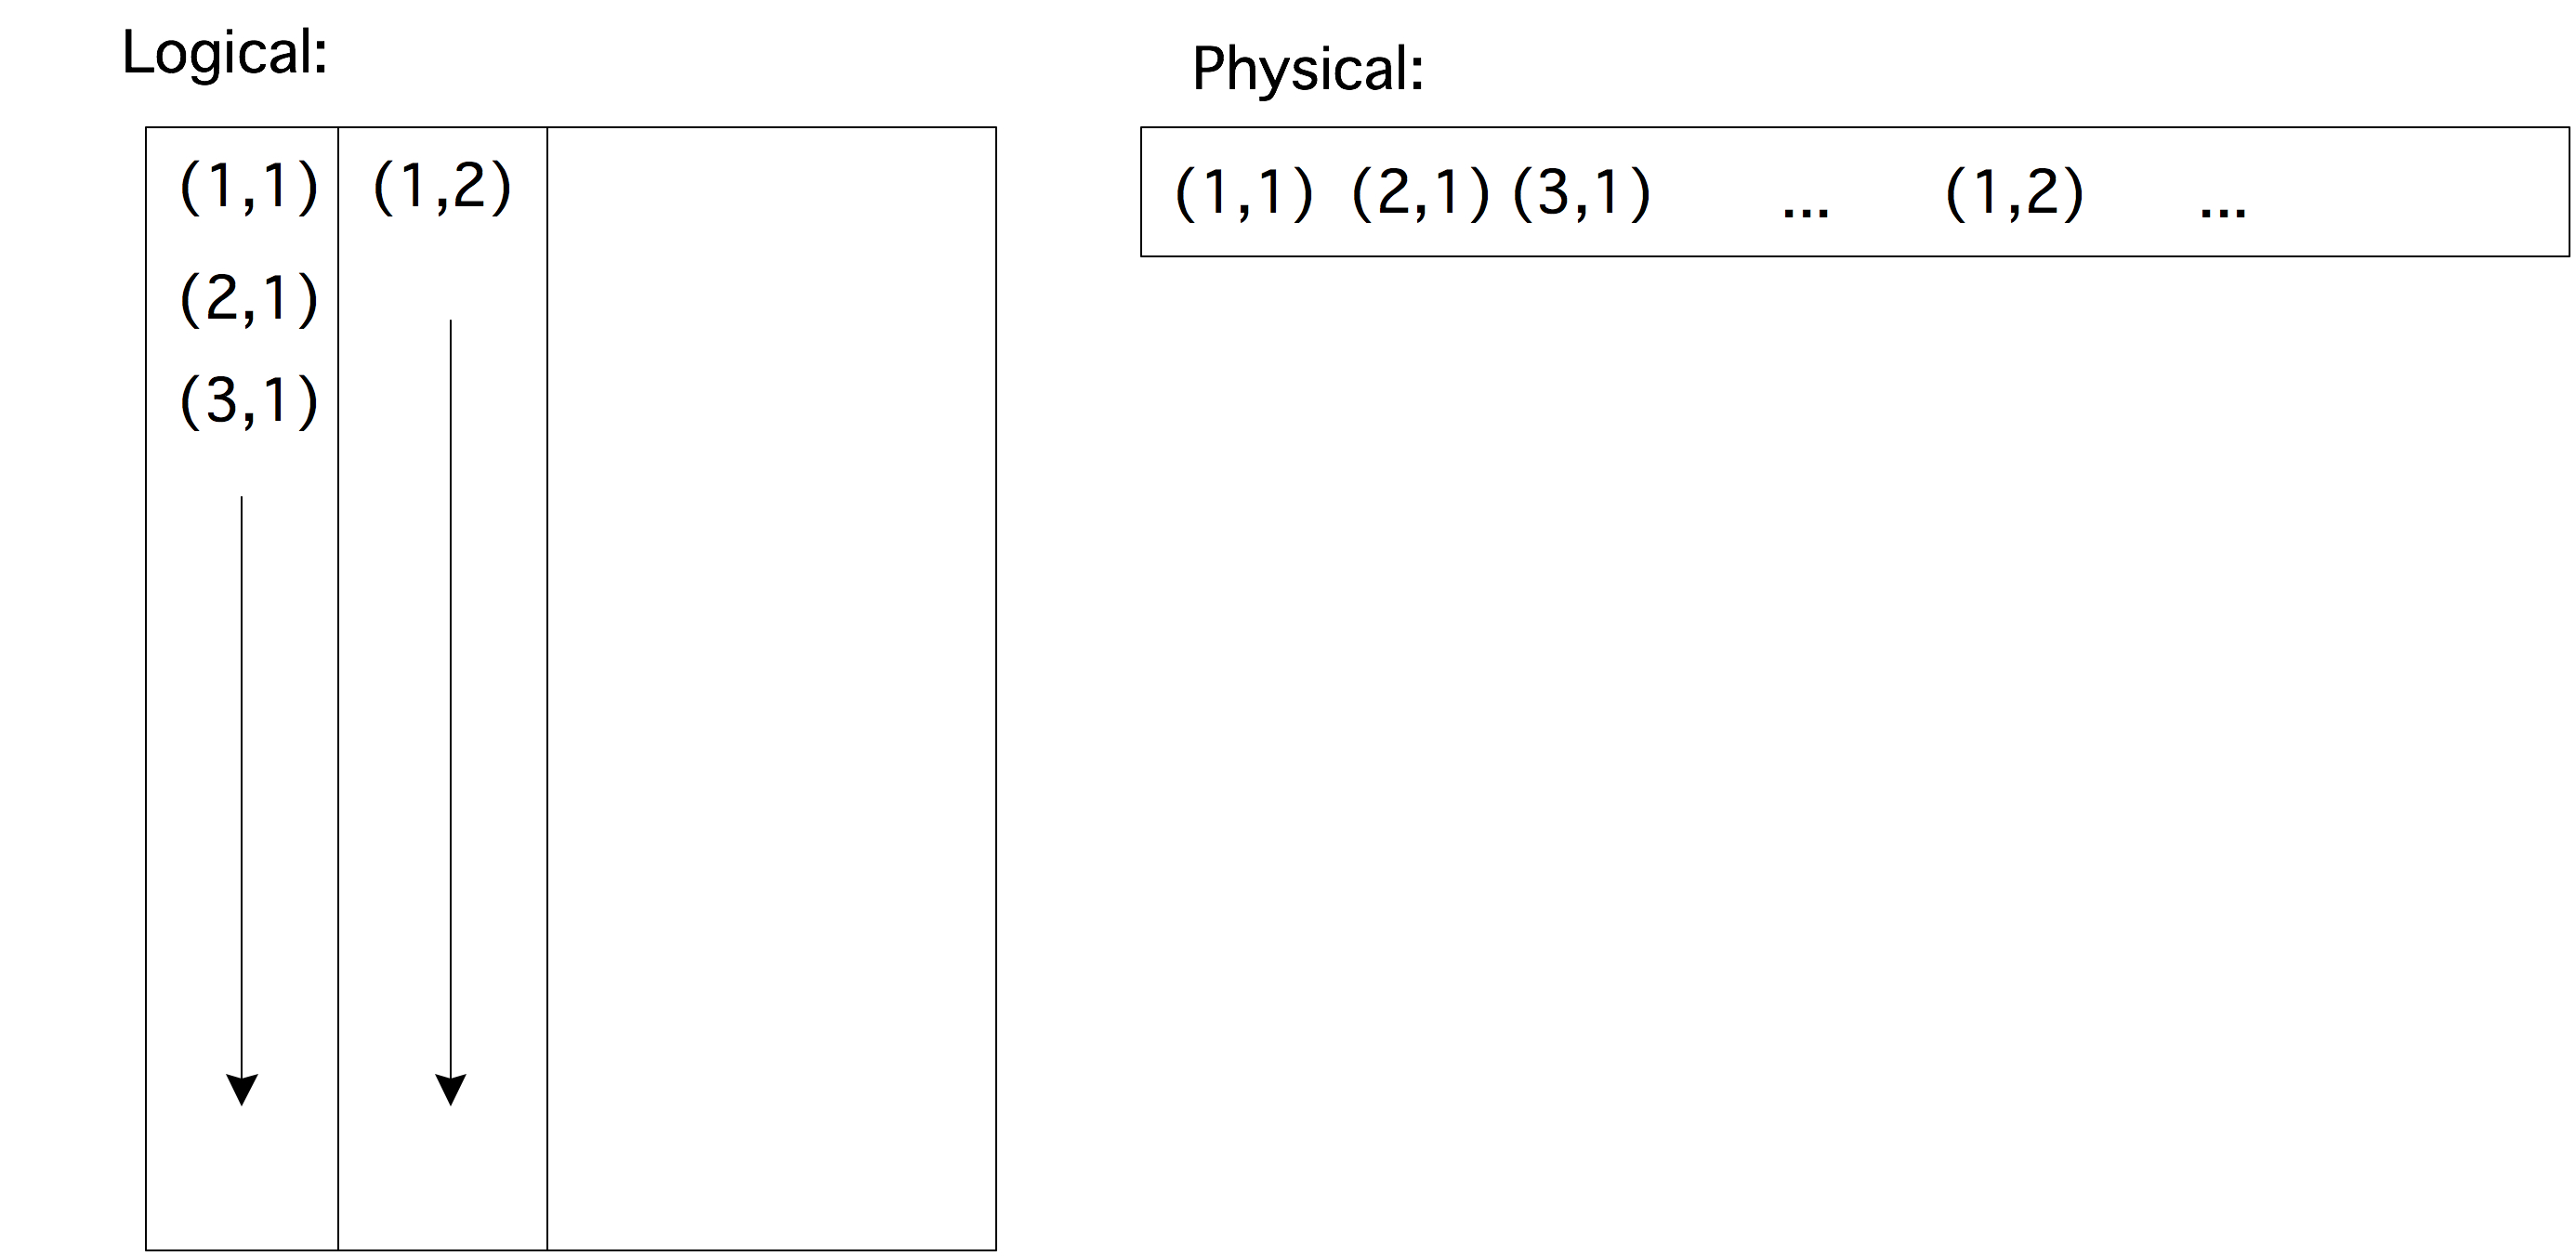
\includegraphics[scale=.14]{graphics-public/densearray}
  \caption{Column-major storage of an array in Fortran}
  \label{fig:densearray}
\end{figure}
This is also described informally as `the leftmost index varies
quickest'.

\Level 2 {Submatrices and the {\tt LDA} parameter}

Using the storage scheme described above, it is clear how to store an
$m\times n$ matrix in $mn$ memory locations. However, there are many
cases where software needs access to a matrix that is a subblock of
another, larger, matrix. As you see in figure~\ref{fig:lda1}
\begin{figure}[ht]
  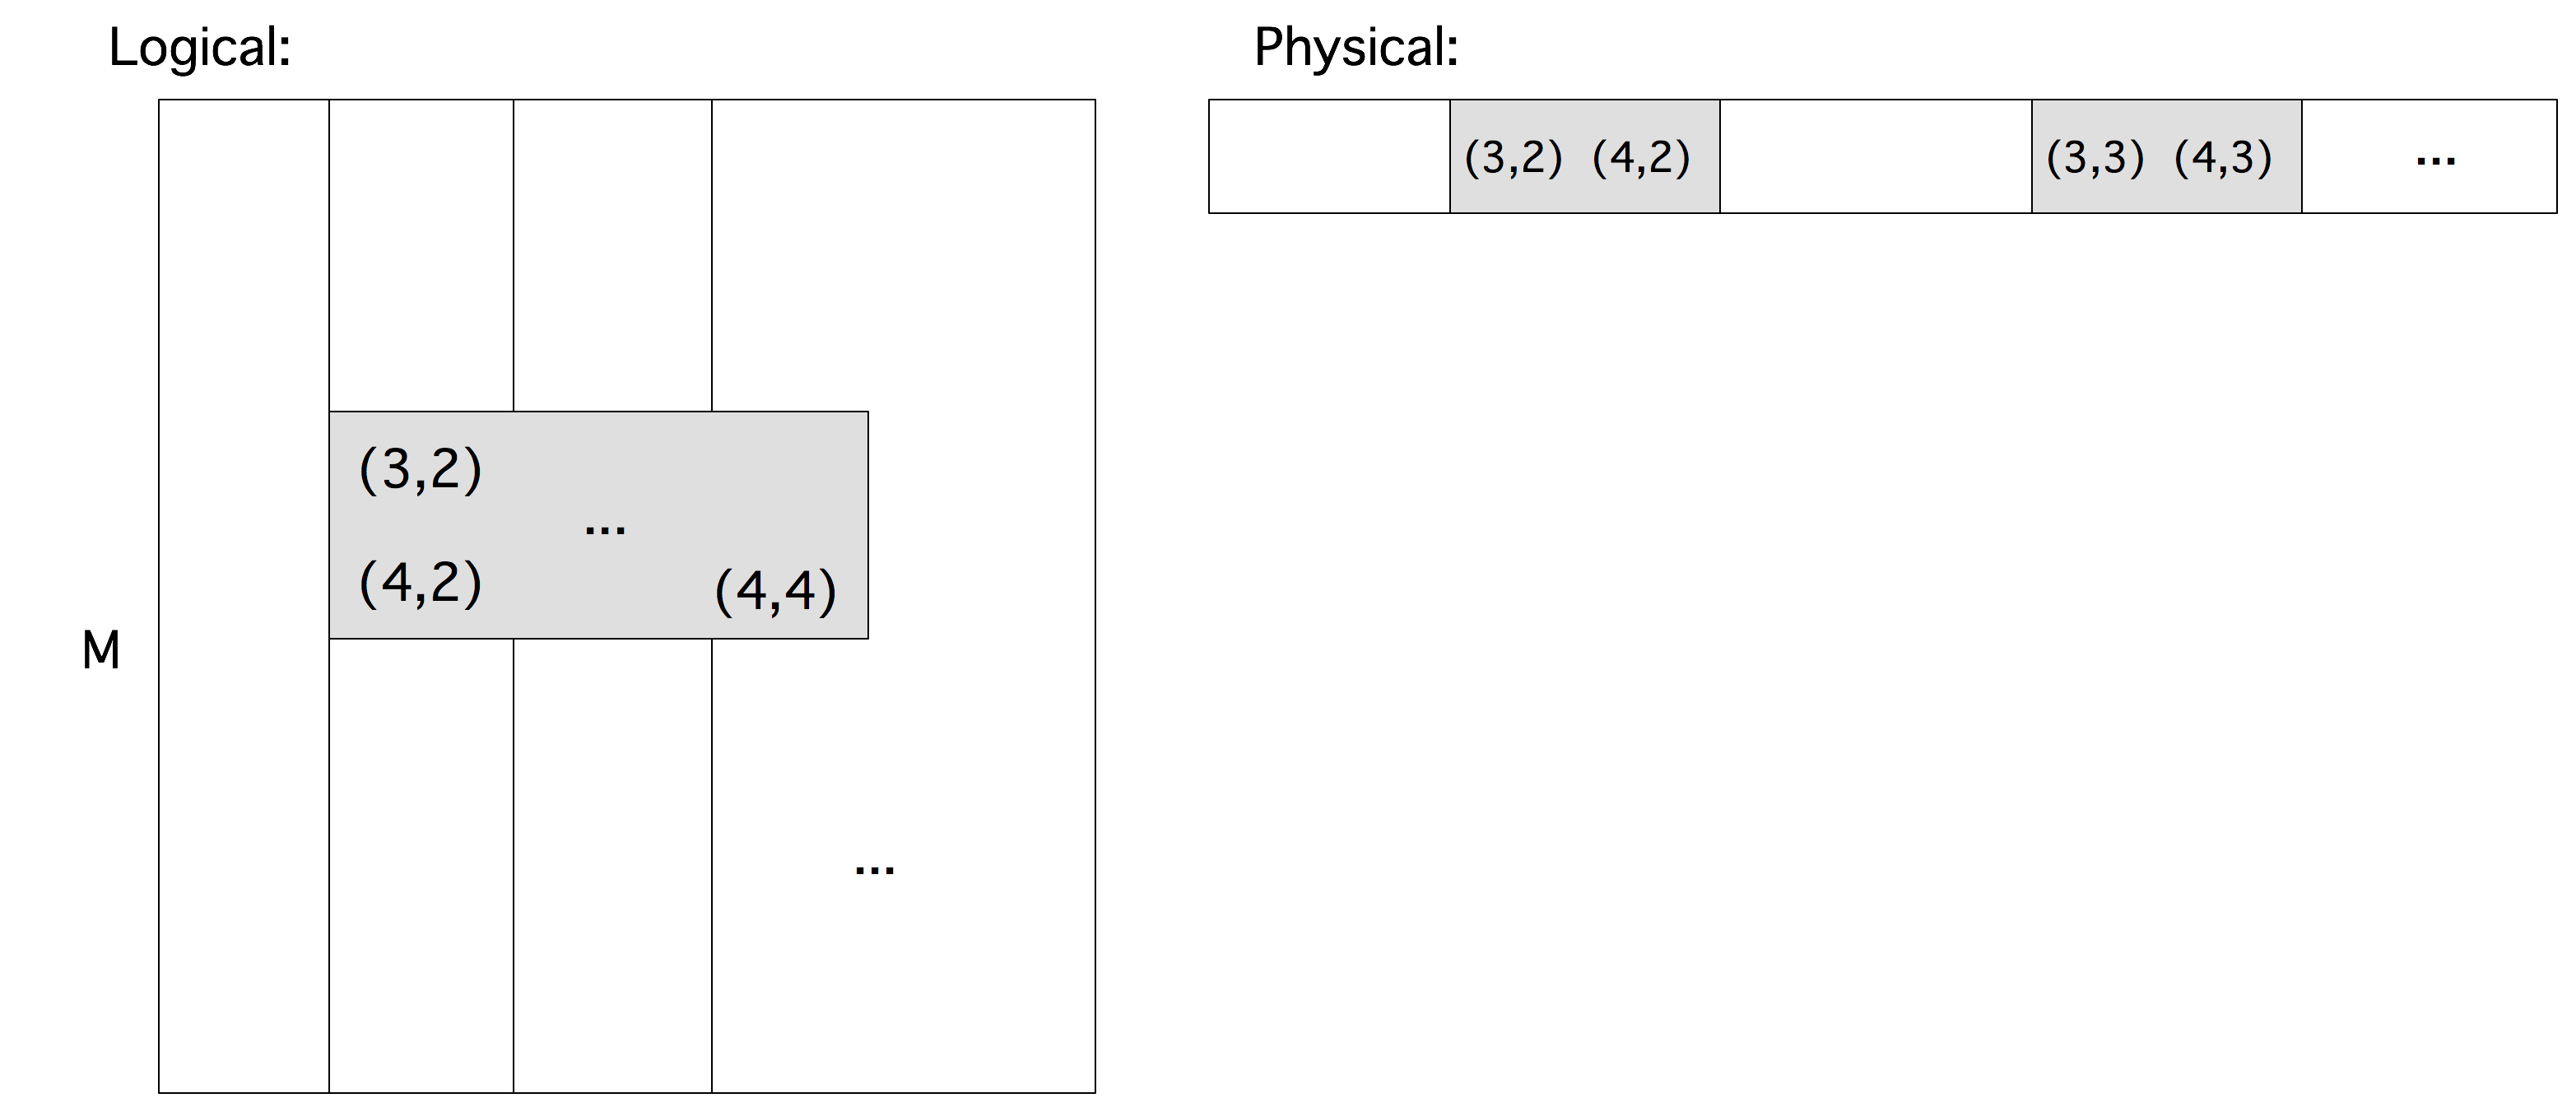
\includegraphics[scale=.14]{graphics-public/denselda}
  \caption{A subblock out of a larger matrix}
  \label{fig:lda1}
\end{figure}
such a subblock is no longer contiguous in memory. The way to describe
this is by introducing a third parameter in addition to~{\tt M,N}: we
let {\tt LDA} be the `leading dimension of~{\tt A}', that is, the
allocated first dimension of the surrounding array. This is
illustrated in figure~\ref{fig:lda2}.
\begin{figure}
  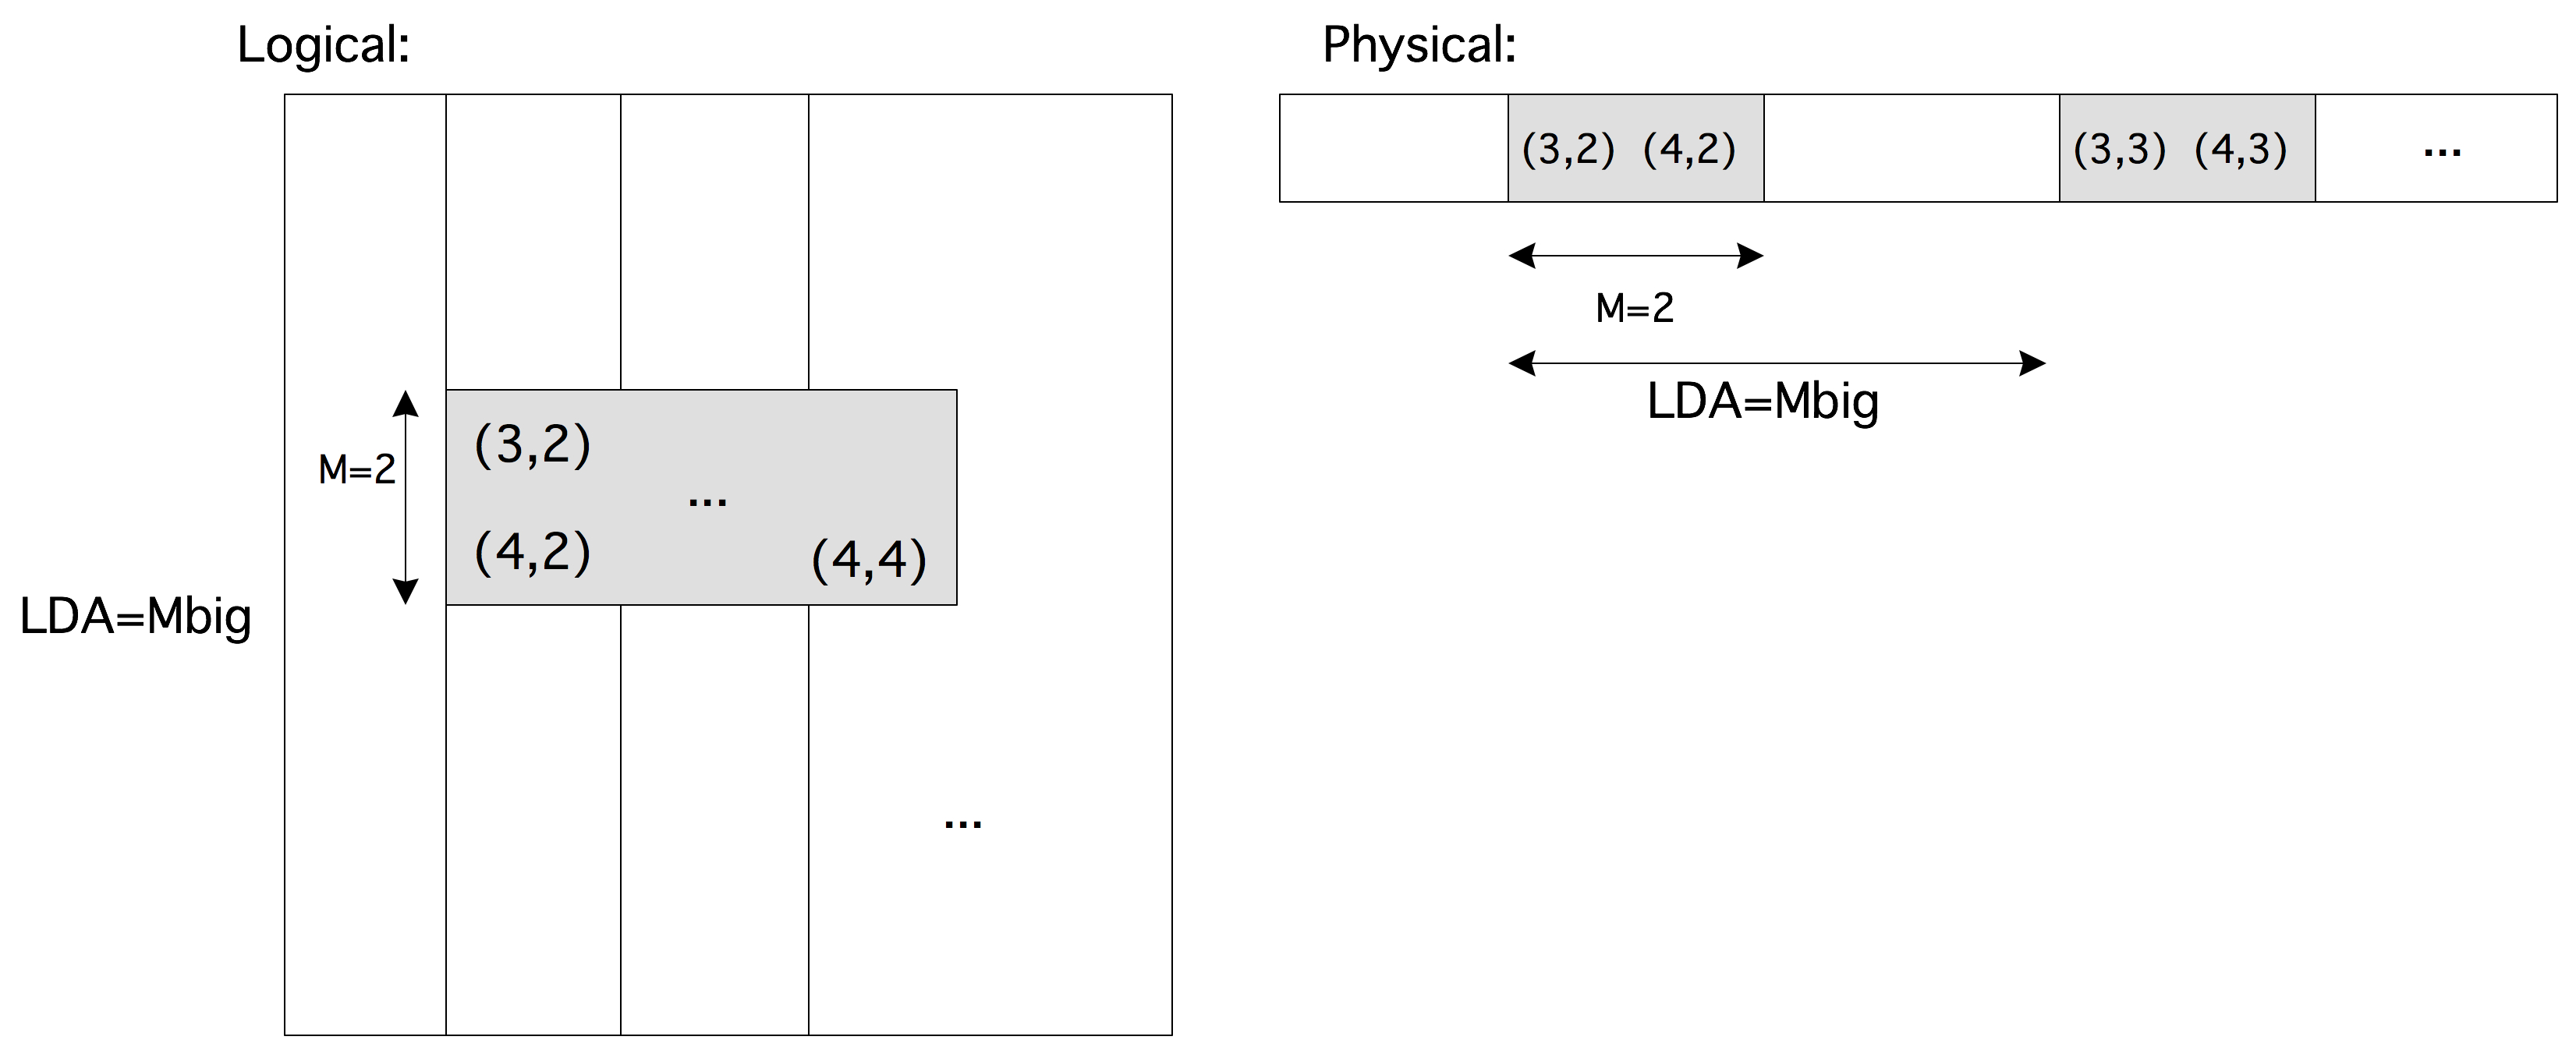
\includegraphics[scale=.14]{graphics-public/denselda2}
  \caption{A subblock out of a larger matrix, using {\tt LDA}}
  \label{fig:lda2}
\end{figure}

\Level 1 {Organisation of routines}
\index{Lapack|(}

Lapack is organized with three levels of routines:
\begin{itemize}
\item Drivers. These are powerful top level routine for problems such
  as solving linear systems or computing an SVD. There are simple and
  expert drivers; the expert ones have more numerical sophistication.
\item Computational routines. These are the routines that drivers are
  built up out of\footnote{Ha! Take that, Winston.}. A~user may have
  occasion to call them by themselves.
\item Auxiliary routines.
\end{itemize}

Routines conform to a general naming scheme: \n{XYYZZZ} where
\begin{description}
\item[X] precision: \n{S,D,C,Z} stand for single and double, single
  complex and double complex, respectively.
\item[YY] storage scheme: general rectangular, triangular, banded.
\item[ZZZ] operation. See the manual for a list.
\end{description}
Expert driver names end on 'X'.

\Level 2 {Lapack data formats}

Lapack and Blas use a number of data formats, including
\begin{description}
\item[GE] General matrix: stored two-dimensionally as \n{A(LDA,*)}
\item[SY/HE] Symmetric/Hermitian: general storage; \n{UPLO} parameter
  to indicate upper or lower (e.g. \n{SPOTRF})
\item[GB/SB/HB] General/symmetric/Hermitian band; these formats use
  column-major storage; in \n{SGBTRF} overallocation needed because of
  pivoting
\item[PB] Symmetric of Hermitian positive definite band; no
  overallocation in \n{SPDTRF}
\end{description}

\Level 2 {Lapack operations}

\begin{itemize}
\item Linear system solving.
Simple drivers: \n{-SV} (e.g., \n{DGESV}) 
Solve $AX=B$, overwrite A with LU (with pivoting),
overwrite B with X.

Expert driver: \n{-SVX}
Also transpose solve, condition estimation, refinement, equilibration
\item Least squares problems.
Drivers: 
\begin{description}
\item[\n{xGELS}] using QR or LQ under full-rank assumption
\item[\n{xGELSY}] "complete orthogonal factorisation"
\item[\n{xGELSS}] using SVD
\item[\n{xGELSD}] using divide-conquer SVD
(faster, but more workspace than \n{xGELSS})
\end{description}

Also: LSE \& GLM linear equality constraint \& general linear model

\item Eigenvalue routines.
Symmetric/Hermitian: \n{xSY} or \n{xHE} (also \n{SP}, \n{SB}, \n{ST})
simple driver \n{-EV}
expert driver \n{-EVX}
divide and conquer \n{-EVD}
relative robust representation \n{-EVR}

General (only \n{xGE})
Schur decomposition \n{-ES} and \n{-ESX}
eigenvalues \n{-EV} and \n{-EVX}

SVD (only \n{xGE})
simple driver \n{-SVD}
divide and conquer \n{SDD}

Generalized symmetric (\n{SY} and \n{HE}; \n{SP}, \n{SB})
simple driver \n{GV}
expert \n{GVX}
divide-conquer \n{GVD}

Nonsymmetric
Schur: simple \n{GGES}, expert \n{GGESX}
eigen: simple \n{GGEV}, expert \n{GGEVX}

svd: \n{GGSVD}

\end{itemize}

\index{Lapack|)}

